\documentclass[../main.tex]{subfiles}
\graphicspath{{\subfix{../../images/}}}

\begin{document}

To make sure that data sent from a device is received on the other side correctly, without errors, error correction must be done to make sure the data is valid. Here are some methods:

\begin{itemize}
    \item \textbf{Parity Checks:} This adds an extra bit (0 or 1) to a piece of data (usually a byte) based on the number of 1s already present. The number of 1s are totalled. Depending on if even or odd parity are agreed upon from the sender and receiver, if the number of 1s is even, the parity bit is 1, for odd parity the parity bit is 1 if the number of 1s is odd. If the receiver's calculated digit is the same as the digit sent, it indicates no error. However, this method can only detect single-bit errors and not multiple-bit errors.
    \item \textbf{Cyclic Redundancy Checks (Checksums, CRCs):} The data bits are added together, processed in a certain predetermined way, and the result (checksum) is appended to the data packet. The receiving device recalculates the checksum on the received data and compares it to the received checksum. If they match, the data is assumed to be error-free. This method is more robust than parity checks.
    \item \textbf{Echo Checks:} The sender sends the data packet and then waits for an exact copy of the packet back from the receiving device. This confirms successful data transfer but introduces a delay due to the back-and-forth communication.
\end{itemize}

\subsection{Parity Blocks}

These are like 2D parity checks. Each byte of data sent will have one bit used for parity, when the digit is calculated horizontally. Then, a whole other byte of data is also sent; with just parity bytes from parity checks from each vertical column.

\begin{figure}[H]
    \centering
    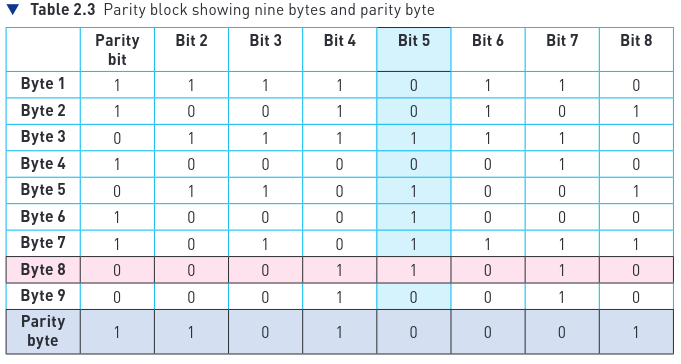
\includegraphics[width=0.7\textwidth]{parity_block.png}
    \caption{From the textbook. "[The table] shows how the data arrived at the receiving end. It is now necessary to check the parity of each byte horizontally (bytes 1 to 9) and vertically (columns 1 to 8). Each row and column where the parity has changed from even to odd should be flagged:"}
    \label{fig:parity_block}
\end{figure}

Figure \ref{fig:parity_block} from the textbook shows this. An extra byte of information is used as parity bits for each column, and each row has one data bit dedicated to storing horizontal parity data. This allows exact errors to be pinpointed (bit flips).

\subsection{Check Digits}

Check digits are another form of error correction; usually involving checking for errors in numbered codes, such as barcodes.

\begin{figure}[h]
    \centering
    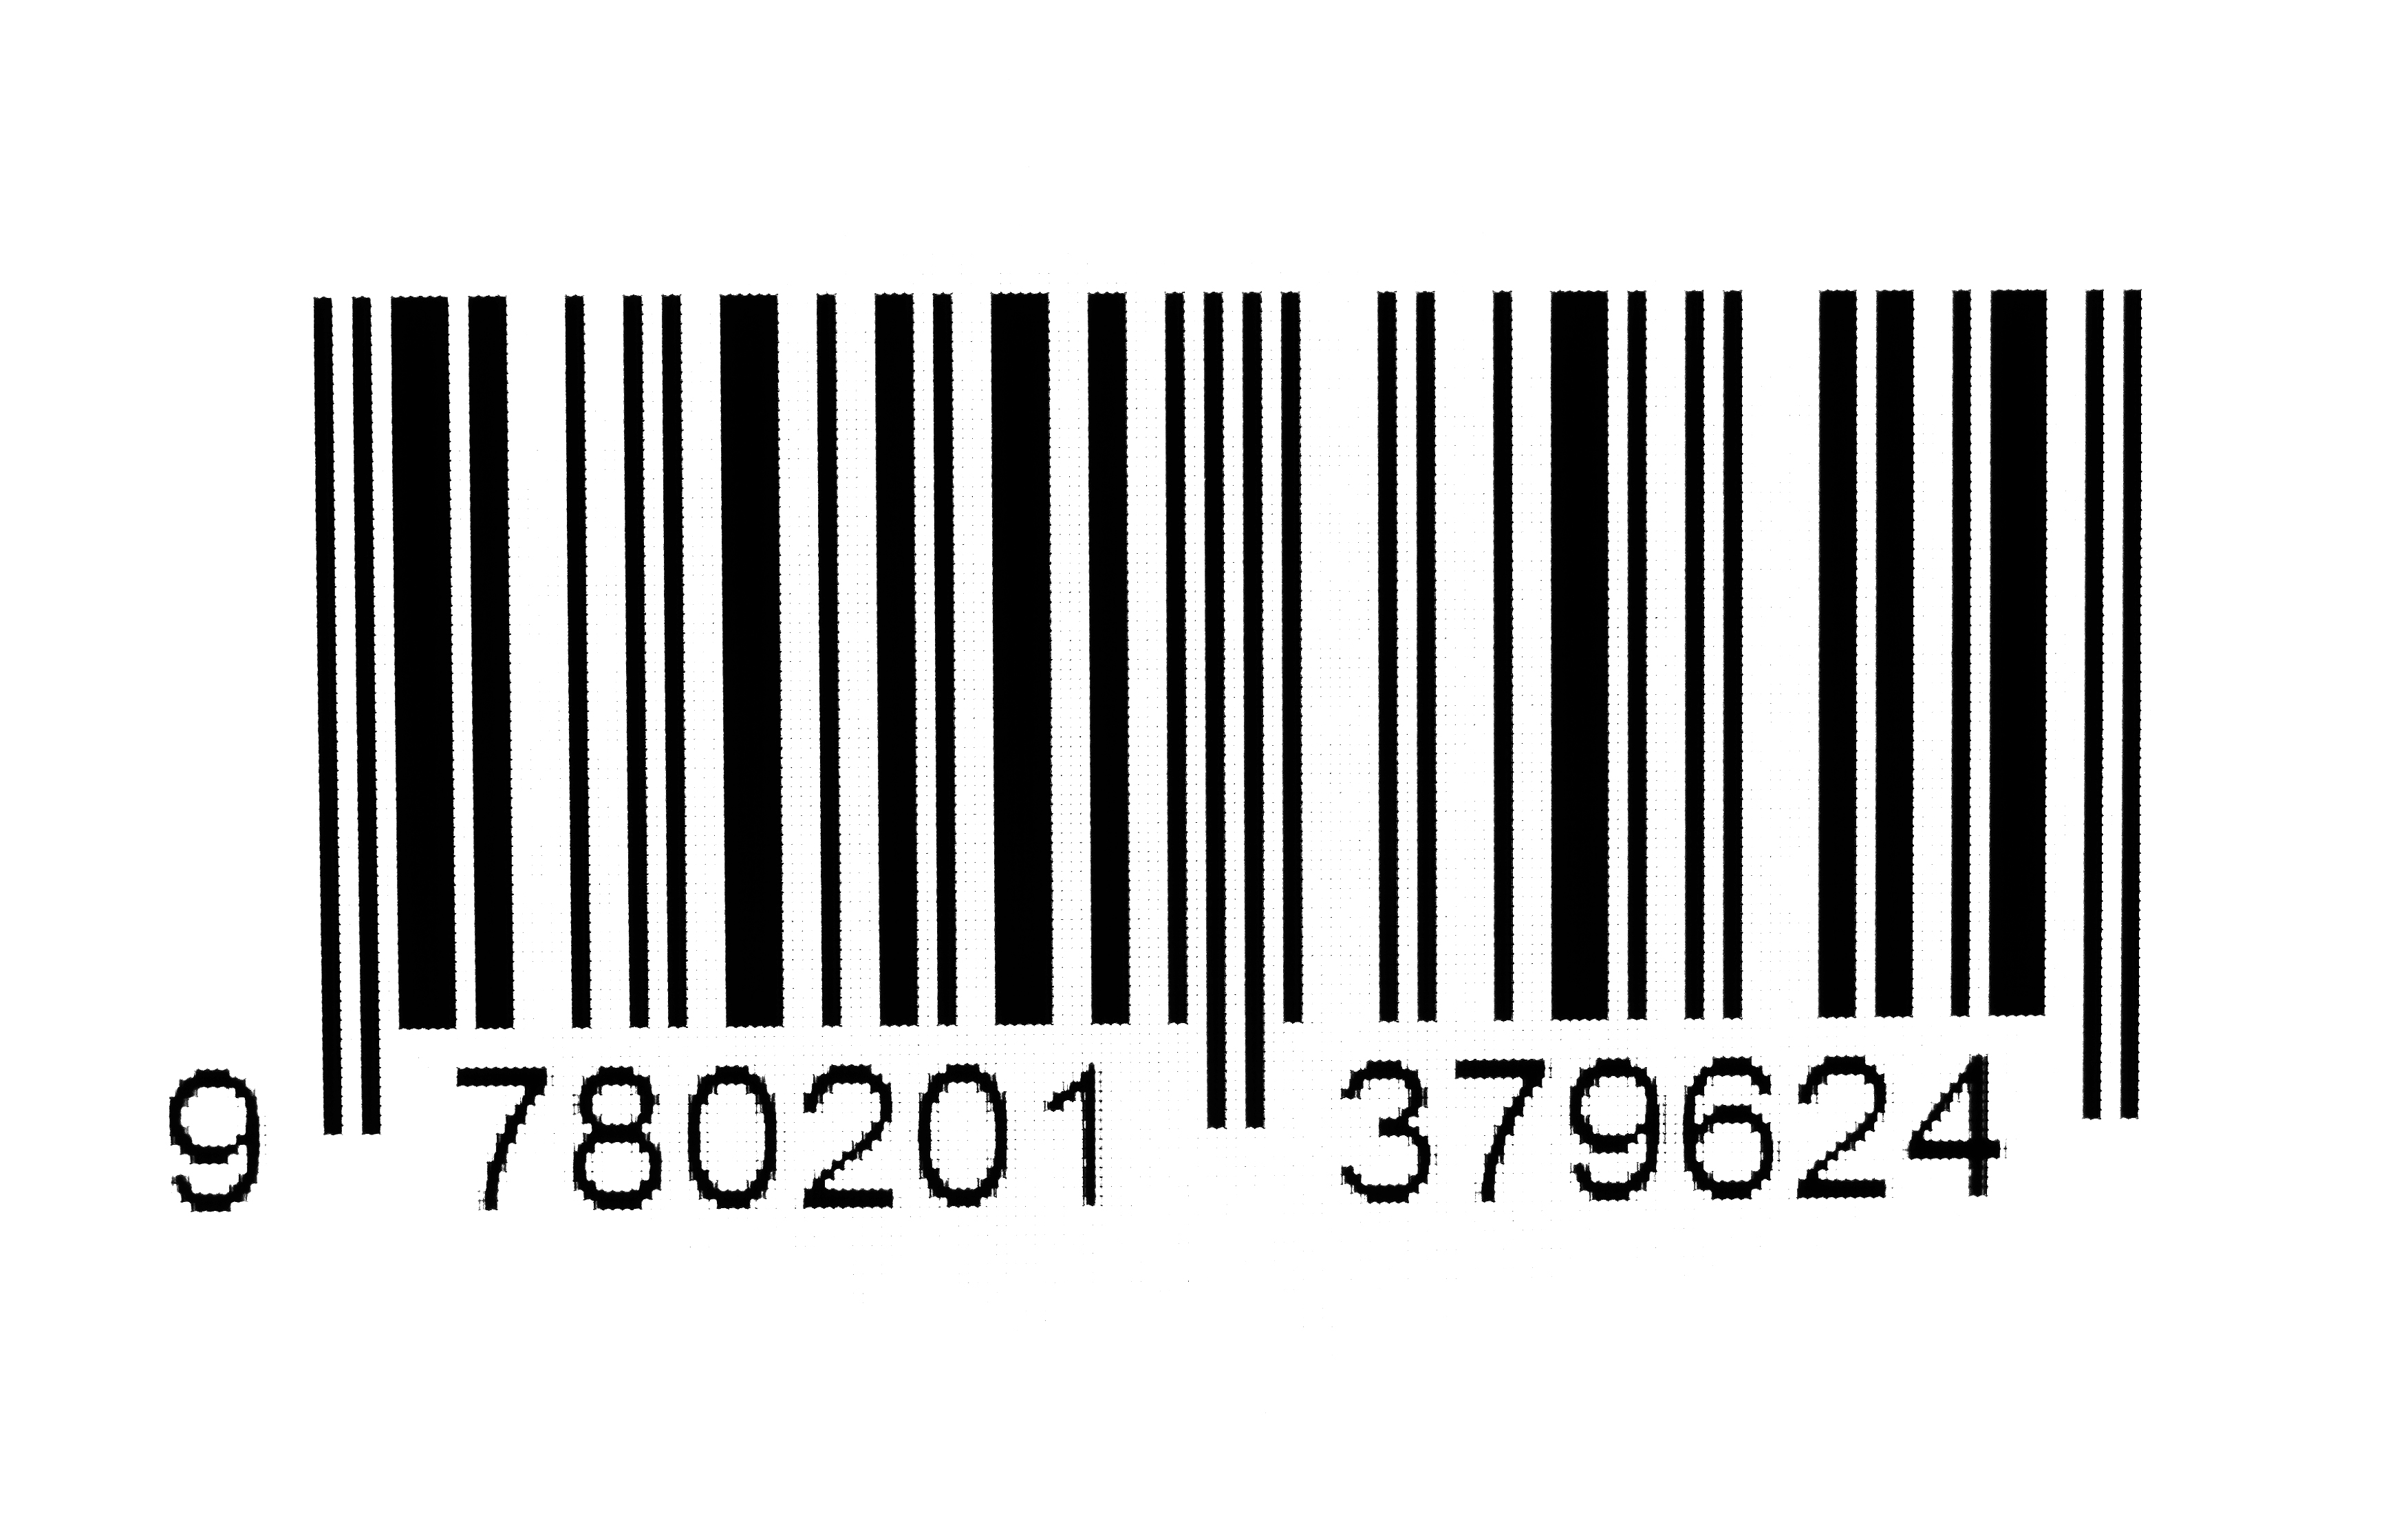
\includegraphics[width=0.6\textwidth]{barcode.png}
    \caption{Barcodes consist of black and white bars that represent decimal numbers; written at the bottom.}
    \label{fig:barcode}
\end{figure}

typically, barcode readers that read these numbers may encouter stains on the physical code and such. Therefore, error correction is needed to make sure the data is not damaged to the point the barcode cannot be read.

This also applies for international standard book numbers, or ISBNs. There is a check digit at the very end of every ISBN code. \emph{Since ISBN-13 and Modulo-11 calculations are not in your syllabus}, you just need to know that barcodes and ISBN codes use check digits.\footnote{They will still be included, just in case if you want to know them, or if your teacher decided to teach it to you.}

\subsubsection{ISBN-13}

To calculate:

\begin{enumerate}
    \item Add all odd digits
    \item Add all even digits, and multipy the result by 3
    \item Add the results from steps 1 and 2, and divide the result by 10
    \item If the remainder is 0, use 0. Otherwise, subtract the remainder from step 3 from 10. This is your check digit.\footnote{As an example, if you got 6 for step 3, your check digit is $10-6$ or 4.}
\end{enumerate}

To verify:

\begin{enumerate}
    \item Add all odd digits
    \item Add all even digits, and multiply the result by 3
    \item Add the results from steps 1 and 2, and divide the result by 10
    \item If the remainder is 0, there is no error.
\end{enumerate}

\subsubsection{Modulo-11}

\emph{Note that Modulo-11 is not at all in your syllabus anymore. However, it may still be taught; if it is assessed internally in your school, as it is still in your textbook, it is still included.} To calculate:

\begin{enumerate}
    \item You must calculate a \emph{Max Weighting}. Take the length of your number data, and add 1 to get your weighting.
    \item Take your first digit, and assign it to your weighting. Assign the next weighting to the max weighting minus one. Assign the next weighting after that to the max weighting minus 2, until you run out of digits.
    \item Multiply each digit by the weight.
    \item Add all the products from step 3 together.
    \item Divide the result from step 4 by 11, and note down the remainder.
    \item Subtract your remainder from 11.\footnote{As an example, if you got 7 from step 5, your remainder is 4}. This is the check digit.
\end{enumerate}

\subsection{Automatic Repeat Requests}

\emph{In short, for small amounts of data, if the data received by the receiver is invalid, it automatically asks the sender to re-send the data}.

This is a system used in networking to make sure the data received by the receiver over the network is valid. Before the data is sent, both sides agree on a timeout. The timeout determines the max time the data can take to be sent. The data is sent, and the timeout (like a stopwatch) begins. If the data is not received before the timeout is over, the data must be re-sent.

\emph{Acknowledgements} are used for the sender and receiver to communicate about where the data is and the integrity of the data. If the data is received correctly, a \emph{positive acknowledgement} is sent back to the sender. If the data is erroneous, a \emph{negative acknowledgement} is sent. If there is no acknowledgement sent, the data is assumed to be lost in transit, and the dat must be resent.

\paragraph{Example}

\begin{itemize}
    \item Tom’s computer wants to send Jerry’s computer a data packet. Tom’s computer establishes a timeout of 10 seconds and sends out the packet.
    \item If Jerry does not send an acknowledgement in time, the communication is cancelled.
    \item If Jerry does get the data, a positive or negative acknowledgement is sent. The process is repeated until there's a positive acknowledgement from Jerry.
\end{itemize}

\end{document}
